\documentclass[../../main.tex]{subfiles} % Use the main document's preamble

\begin{document}
\chapter{Introduction test}

This document will contain ALLLLL the notes I take on everything I learn. I will try to keep it as organized as possible, but I can't promise anything.

\section{Latex settings}
Latex is a pain to use sometimes. Currently, with the setup i have, i have to do some magic rituals to get the subfiles to compile correctly. I have to have a \texttt{.latexmkrc} file in the root directory of the project, se next section, and the following sections settings in the \texttt{settings.json} file in vscode.

The main.tex file typically compiles fine, but the subfiles don't compile correctly after compiling the main file unless you do the following. (1) compile main file (ctrl-s will build automatically), (2) go to subfile and change the path from \verb|\document class[../../main.tex]| to \verb|\document class[../main.tex]{subfiles}|, the sub file will build and send output to a weird spot, and i think through an error, that's fine. (3) change the path back to \verb|\documentclass[../../main.tex]| and the subfile will build correctly, with its pdf in the same folder as the subfile.tex. 

This should be fixable, but i haven't figured it out yet.

Update, on july 29 2024 that stopped working for some reason. On a whim i decided to copy the project into overleaf and try it, and it just worked, so i'm going to switch to Overleaf, which is probably better in most ways except it's offline access. honestly though, im at the point where i need constant internet for so much anyway, that findng a case where that's gonna be the issue is hopefully not gonna come up much. 
\subsection{latexmkrc}
the following is the content of the \texttt{.latexmkrc} file (as of 6/26/2024):
\begin{lstlisting}
    # .latexmkrc
use File::Basename;

# Custom subroutine to compile subfiles
add_cus_dep('tex', 'pdf', 0, 'subfile_pdf');
sub subfile_pdf {
    my ($base_name, $path) = fileparse(shift);
    my $dir = $path ? "$path/" : "";

    system("latexmk -pdf -aux-directory=out $dir$base_name.tex");
    return 0;
}

# Hook into LaTeXmk's clean routine to remove auxiliary files
add_cus_dep('tex', 'clean', 0, 'clean_aux_files');
sub clean_aux_files {
    my ($base_name, $path) = fileparse(shift);
    my $dir = $path ? "$path/" : "";

    system("rm -f out/$base_name.*");
    return 0;
}

# Ensure LaTeXmk knows to clean auxiliary files on 'latexmk -C'
push @clean_ext, qw(aux log out toc fdb_latexmk fls nav snm vrb xdv);

# Output directory for auxiliary files
$aux_dir = 'out';
\end{lstlisting}

that script placed in the root directory of the project will allow latexmk to compile subfiles and clean auxiliary files. the pdfs will be in the root directory, while the auxiliary files will be in the \texttt{out} directory. cleaning the project will remove all auxiliary files named "main" but not the pdfs. clean doesn't clean the subfiles auxiliary files currently. the preview pdf button in vscode will not work with the aux files with this setup, but the pdfs will update if opened manually. 

\subsection{settings.json}
as of 6/26/2024, the following is the content of the \texttt{settings.json} file:
\begin{lstlisting}
    {
        "workbench.colorTheme": "Visual Studio Dark",
        "editor.showFoldingControls": "always",
        "security.workspace.trust.untrustedFiles": "open",
        "editor.inlineSuggest.enabled": true,
        "julia.symbolCacheDownload": true,
        "wolfram.command": [
            "`kernel`",
            "-noinit",
            "-noprompt",
            "-nopaclet",
            "-noicon",
            "-nostartuppaclets",
            "-run",
            "Needs[\"LSPServer`\"];LSPServer`StartServer[]"
        ],
        "wolfram.kernel": "C:\\Program Files\\Wolfram Research\\Mathematica\\13.3\\WolframKernel.exe",
        "git.openRepositoryInParentFolders": "always",
        "editor.minimap.enabled": false,
        "julia.enableTelemetry": false,
        "github.copilot.advanced": {},
        "jupyter.askForKernelRestart": false,
        "editor.tabCompletion": "on",
        "editor.formatOnPaste": true,
        "python.analysis.autoSearchPaths": true,
        "python.autoComplete.extraPaths": [
            "Z:\\home\\Vandy\\code\\vandyCode\\MyPackages"
        ],
        "python.analysis.extraPaths": [
            "Z:\\home\\Vandy\\code\\vandyCode\\MyPackages"
        ],
        "explorer.confirmDelete": false,
        "explorer.confirmDragAndDrop": false,
        "julia.lint.run": true,
        "security.allowedUNCHosts": [
            "srsrv1"
        ],
        "jupyter.debugJustMyCode": false,
        "python.defaultInterpreterPath": "C:\\Users\\micha\\anaconda3\\python.exe",
        "jupyter.stopOnFirstLineWhileDebugging": false,
        "jupyter.showVariableViewWhenDebugging": true,
    
        "latex-workshop.latex.recipes": [
            {
                "name": "latexmk",
                "tools": [
                    "latexmk"
                ]
            }
        ],
        "latex-workshop.latex.tools": [
            {
                "name": "latexmk",
                "command": "latexmk",
                "args": [
                    "-synctex=1",
                    "-interaction=nonstopmode",
                    "-file-line-error",
                    "-pdf",
                    "%DOC%"
                ]
            }
        ],
        "latex-workshop.latex.autoBuild.run": "onSave",
        "latex-workshop.viewer.pdf.tab.editorGroup": "both"
    }
\end{lstlisting}

and things are working well.

\section{Mathematica settings}
To change mathematica's annoyingly large margins , you can fight with the inheritance system and options inspector, with the option CellMargins. Or you can edit the package stylesheet. you aren't allowed to edit the default stylesheet, so you have to make a new one and put it in the appropriate directory.

\begin{lstlisting}
    CopyFile @@ (FileNameJoin[{#, "SystemFiles", "FrontEnd", 
      "StyleSheets", 
      "Package.nb"}] & /@ {$InstallationDirectory, $UserBaseDirectory})
\end{lstlisting}

will copy the default package stylesheet to the user directory. you can then edit the stylesheet to change the margins. The sheet looks like this:


\begin{figure}[H]
    \centering
    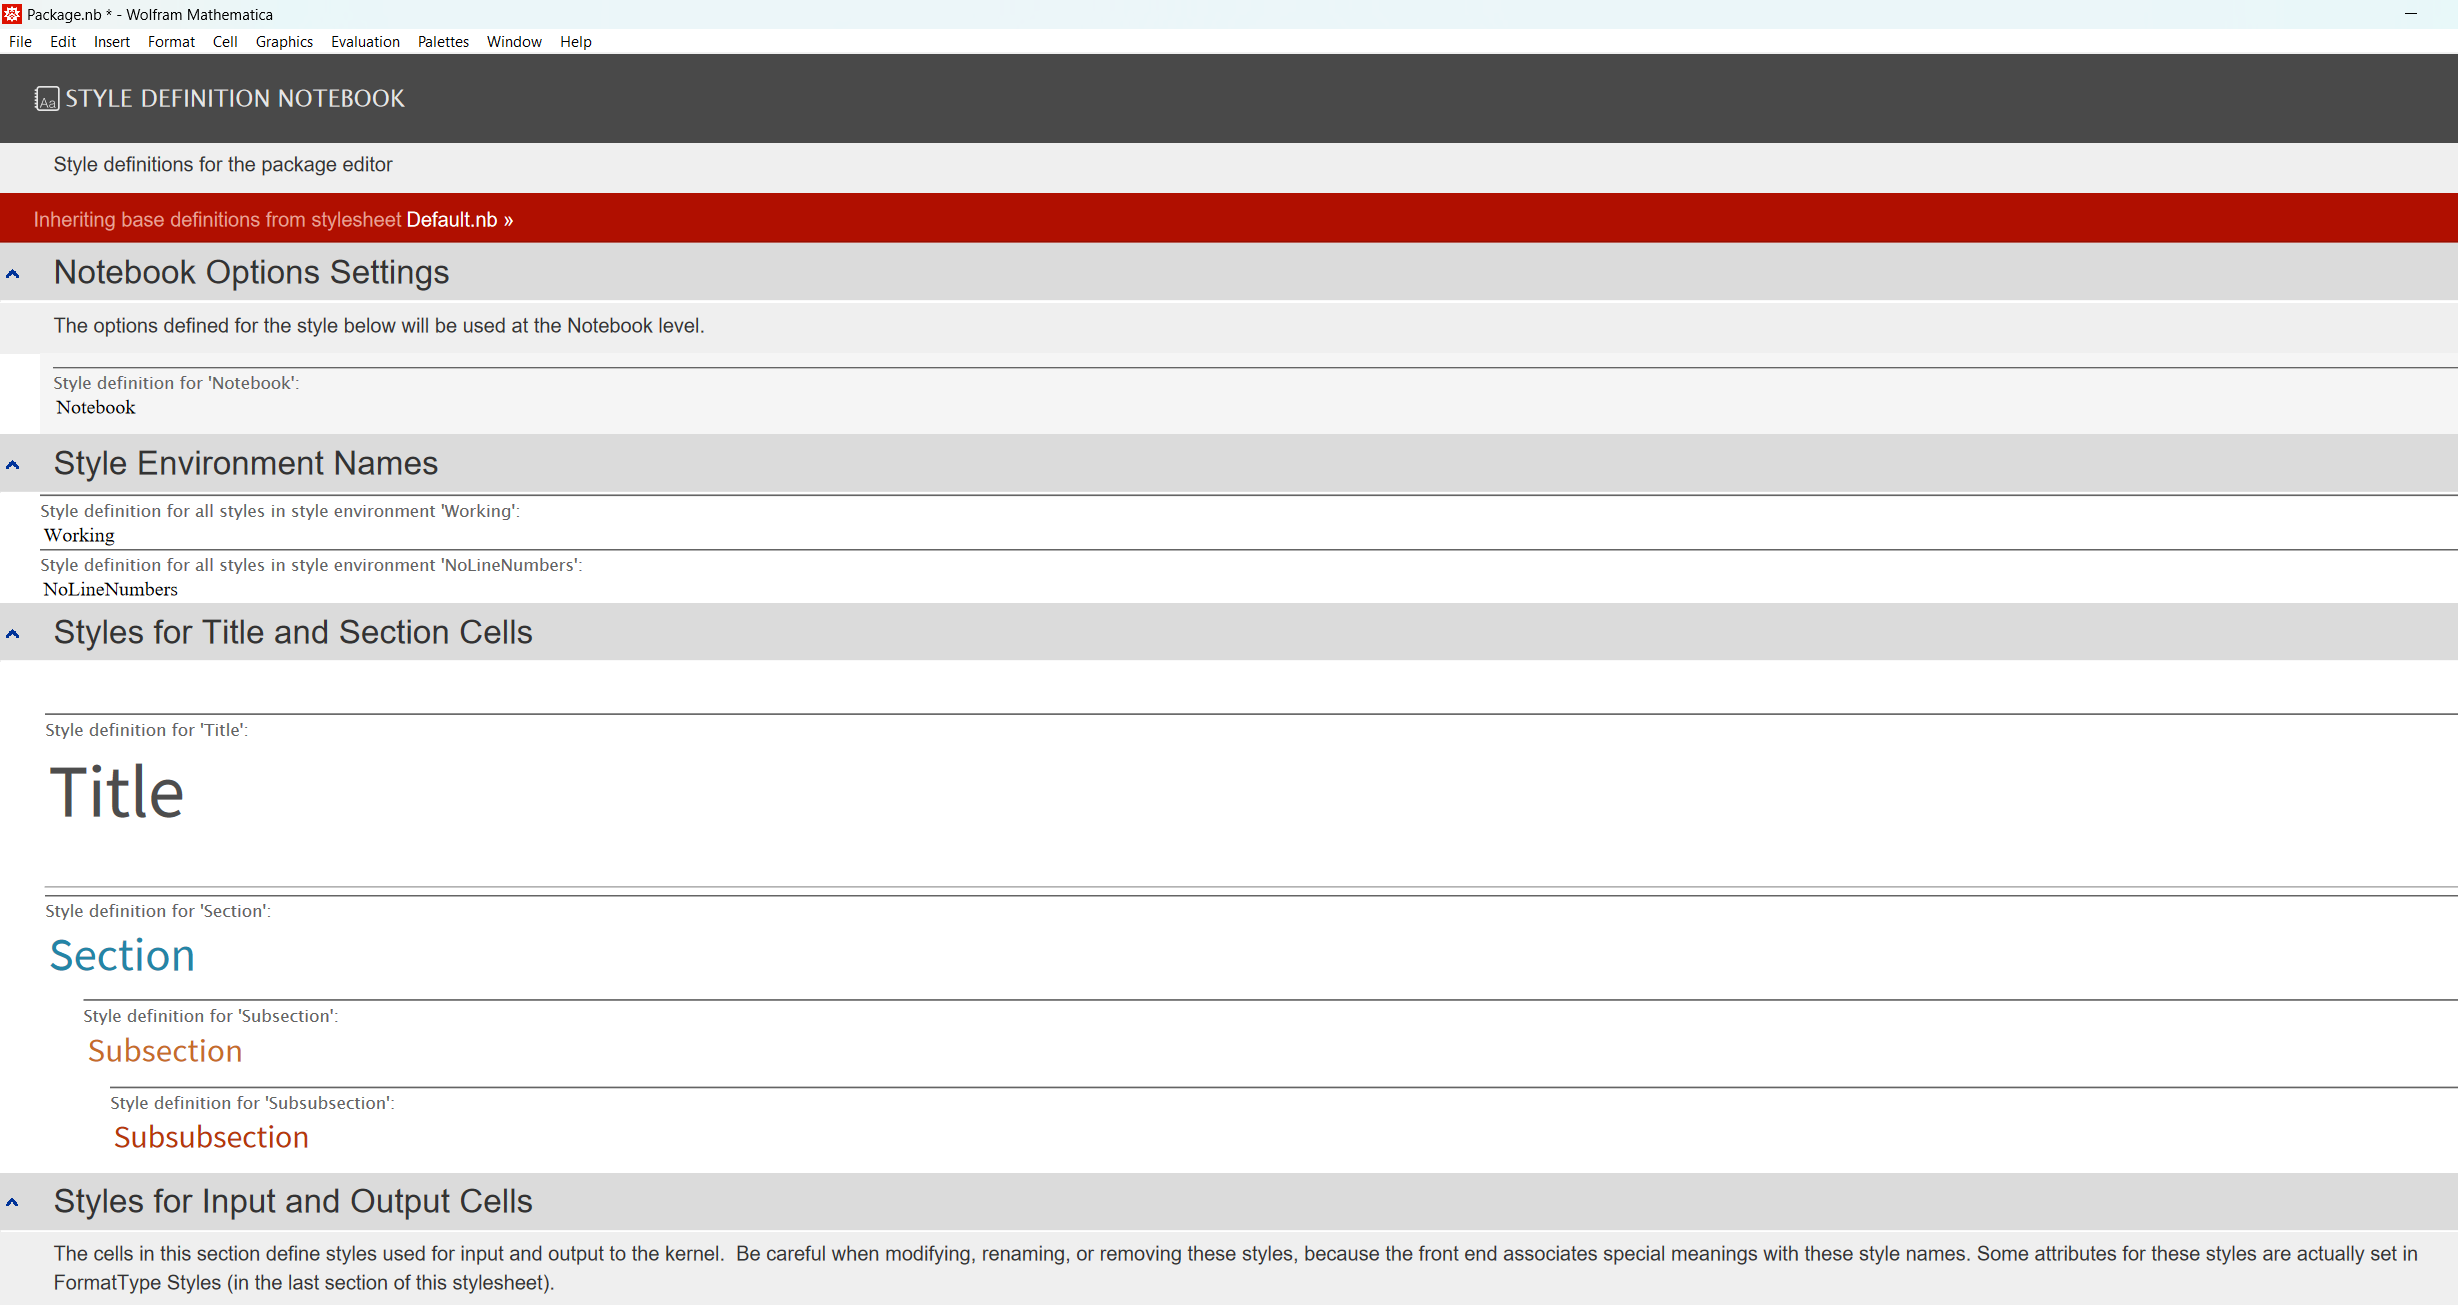
\includegraphics[width=0.8\textwidth]{Chapters/intro/stylesheet.png}
    \caption{The stylesheet}
    \label{fig:stylesheet}
\end{figure}

To edit the style of a type of cell, select the cell, such as the "Title" cell, and Show the Cell Expression via ctrl+shift+E. You can then edit the cell's style. For example, to change the margins of the title cell, you can change the margins in the cell expression by adding the option CellMargins$\rightarrow$\{\{left,right\},\{bottom,top\}\}.

Another fun fact, ifasdfa 

\section{Git}
you can use the following command to remove the specific safe directory directly from the terminal: 
\begin{verbatim}
    git config --global --unset safe.directory "//srsrv1/lab/home/Vandy/Latex/EverythingTwo"
\end{verbatim}
To initialize a repo in an existing folder and link it to a remote repo do
\begin{verbatim}
    cd path/to/your/folder
    git init
    git add .
    git commit -m "Initial commit"
    git remote add origin 
    https://github.com/username/repository.git 
    or git@github.com:username/repository.git
    git push -u origin master
\end{verbatim}
If SSH is being used, use the git@ version, (and note the semicolon after .com)


\end{document}
